\documentclass{beamer}
\usepackage{tikz}
\usepackage{smartdiagram}
\usepackage{xmpmulti}
\usepackage{pgfpages}


%\setbeameroption{show notes}
%\setbeameroption{show notes on second screen=right}
\mode<presentation> {
  \usetheme{Warsaw}
  % ou autre ...

  \setbeamercovered{transparent}
  % ou autre chose (il est également possible de supprimer cette ligne)
}


\usepackage[spanish]{babel}
\usepackage[latin1]{inputenc}
\usepackage{times}
\usepackage[T1]{fontenc}
\usepackage{tikz}
\pgfdeclareimage[height=1cm]{le-logo}{logouni}
\logo{\pgfuseimage{le-logo}}
\setbeamertemplate{footline}[frame number]


%%%%%%%%%%%%%%%%%%%%%%%%%%%
\title[Redes LSTM para el reconocimiento de voz
aplicado a un conjunto de d�gitos] 
{Redes LSTM para el reconocimiento de voz
	aplicado a un conjunto de d�gitos}
%\subtitle {ne compléter que si l'article possède un sous-titre}

\author[V�ctor Jes�s Sotelo Chico] 
{Victor Jesus Sotelo Chico\inst{1}}

\institute[]
{
  \inst{1}%
  Universidad Nacional de Ingenier�a\\

  }

\date[Seminario de Tesis II] 
{Seminario de Tesis II}



\begin{document}


\begin{frame}
  \titlepage
\end{frame}

\begin{frame}{Contenido}
  \tableofcontents
\end{frame}

\section{Introducci�n}
\begin{frame}{Introducci�n}
	Las se�ales de voz proveen una gran cantidad de informaci�n a trav�s del tiempo, el estudio de estas ha permitido el desarrollo de sistemas de reconocimiento de voz.

\end{frame}
\section{Objetivos}

\begin{frame}{Objetivos}
  %\includegraphics[scale=0.3, angle=-90]{construction-process}
  \begin{itemize}
  	\item Conocer el proceso involucrado en el habla humana.
	\item Estudiar procesamiento de las se�ales de voz.
	 \item Dise�ar una red neuronal capaz de reconocer un conjunto de audios de n�meros.
	\item Mostrar los resultados obtenidos y explicarlos bas�ndonos en la teor�a estudiada.
  \end{itemize}
\end{frame}


\section{Marco Te�rico}

\subsection{Redes Neuronales}
\begin{frame}{Redes Neuronales Artificiales}
Estas redes toman como inspiraci�n la arquitectura
del cerebro para la construcci�n de sistemas inteligente.
Actualmente son la base para el desarrollo de la inteligencia artificial.

\end{frame}
\begin{frame}{Comparaci�n neuronas biol�gicas y artificiales}
	\begin{figure}
		\centering
		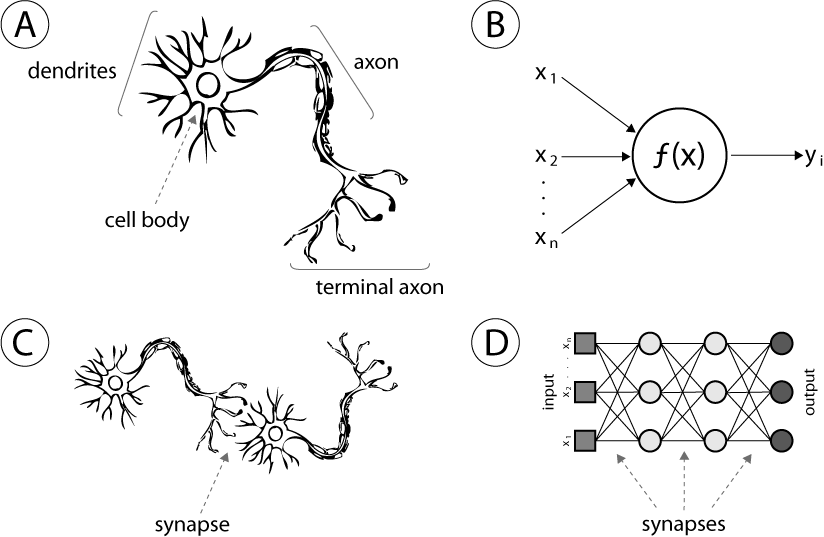
\includegraphics[width=0.6\textwidth]{figures/ANN.png}
		\caption{Redes neuronales biol�gicas y artificiales }
			\label{neuronas}
	\end{figure} 
\end{frame}

\begin{frame}{Redes neuronales Prealimentadas}
Es un tipo de red neuronal m�s simple que existe. Esta red puede clasificarse en:

\begin{itemize}
	\item Perceptron simple
	\item Perceptron Multicapas
	\item Redes neuronales convolucionales
\end{itemize}
\end{frame}
\begin{frame}{Esquema Redes neuronales Prealimentadas}
\begin{figure}[H]
	\centering
	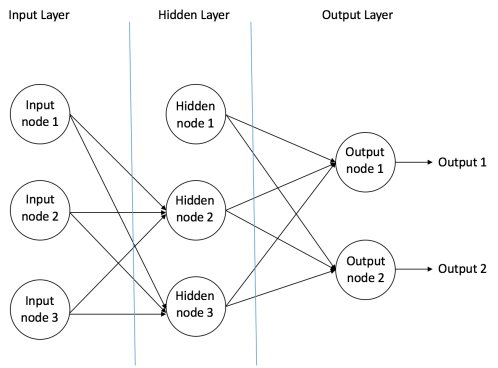
\includegraphics[width=0.7\textwidth]{figures/esquemaff.png}
	\caption{Esquema de Redes Neuronales Prealimentadas }
	\label{neuronasredes}
\end{figure} 
\end{frame}
\begin{frame}{Back Propagation}
	\begin{figure}[H]
		\centering
		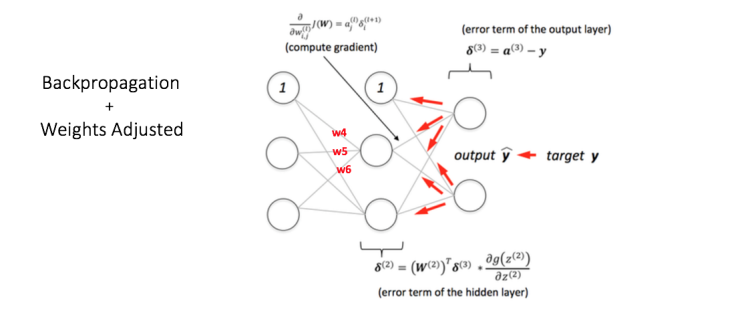
\includegraphics[width=0.8\textwidth]{figures/backp.png}
		\caption{Propagaci�n hacia atr�s}
		\label{backpropagation}
	\end{figure} 
\end{frame}
\begin{frame}{Redes Neuronales Convolucionales(CNN)}
Las CNN son un tipo de redes neuronales especiales para procesar datos
como im�genes. La primera CNN fue creada por Yann LeCun. 

\end{frame}

\begin{frame}{Capas de una red neuronal convolucional}
	\begin{itemize}
		\item Input Layer
		\item Convolutional Layer
		\item Pooling Layer
		\item Fully Conected Layer
		\item Output Layer
	\end{itemize}
	
\end{frame}

\subsection{Redes LSTM}
Las Redes LSTM o Long Short Term Memory son un tipo de redes neuronales recurrentes.


\section{M�todos de Optimizaci�n}

\begin{frame}{Gradiente de Descenso}
	La gradiente de descenso es una forma de minimizar la funci�n de costo $J(\theta)$ parametrizada por los par�metros $\theta \in\Re^{d}$.
	\begin{figure}[H]
		\centering
		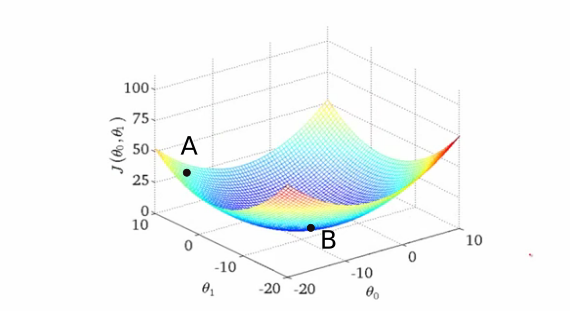
\includegraphics[width=0.6\textwidth]{figures/gd.png}
		\caption{Gradiente de descenso}
		\label{image}
	\end{figure}
\end{frame}
\begin{frame}{Variantes de la Gradiente de Descenso}
	Existen 3 variantes de la gradiente de descenso:
	\begin{itemize}
		\item Batch gradient descent
		\item Stochastic gradient descent
		\item Mini-batch gradient descent
	\end{itemize}

\end{frame}


\section{Conclusiones y Trabajos Futuros}

\begin{frame}{Conclusiones}
	\begin{itemize}
		\item Los m�todos de optimizaci�n Adam y RMSprop obtuvieron los mejores
		resultados de precisi�n en ambas pruebas.
		\item A pesar de que el m�todo de optimizaci�n Adam fue propuesto a partir
		del RMSprop. Adam fue superado en algunas de pruebas realizadas.
		\item Adam es el m�todo que tiene un decaimiento m�s acelerado al calcular el
		error en la funci�n de costo cross-entropy.

	\end{itemize}
\end{frame}

\begin{frame}{Conclusiones}
	\begin{itemize}
		\item Entre los m�todos adaptativos Adam, RMSprop y Adagrad . Solo este
		�ltimo obtuvo los peores resultados, esto se debi� a su dificultad de
		trabajar con la suma de las gradientes al cuadrado lo cual poco a poco
		redujo su tasa de aprendizaje.
		\item El RMSprop como una mejora del Adagrad, obtuv� mejores resultados
		que este �ltimo. Esto debido a que RMSprop trabaja con el promedio
		de la ra�z de la gradiente anterior y tasas de decaimiento para controlar
		el problema de la disminuci�n de la tasa de aprendizaje del m�todo
		Adagrad.
	\end{itemize}
\end{frame}

\begin{frame}{Trabajos Futuro}
	\begin{itemize}
		\item Correcto dise�o de una red neuronal convolucional.
		\item Obtener resultados con distintos hardwares.
		\item Realizar una implementaci�n m�s interactiva.
	\end{itemize}
\end{frame}

\end{document}